\section{Regular boundaries and ordered erosion}\label{rg:section}

The visible boundary from Section~\ref{if:section} is a Jordan base
with finitely many signed slits. We now replace it by one deterministic
regular boundary. The replacement must work for every sufficiently
nearby realizable stopping transcript, even though those transcripts
can have different examined sets. This uniform local statement is what
will permit the finite probability cover in Section~\ref{de:section}.

\subsection{Local replacement and the reduction to spin means}

Choose a source contour $S_0$ and a square test contour $J$ in the free
region between the entire permitted stopping band and the target.
Choose their positive collars so that $J$ is an admissible cut between
$S_0$ and the target, in the sense of Definition~\ref{tr:admissible}.
All modifications of the facing boundary occur on the band side of
$S_0$. For each fixed distant-wall assignment, the two laws in an
ordered insertion therefore have the same conditional continuation
from $S_0$ toward the target. Write
\begin{equation}\label{if:line-mean}
                 M_J^\delta=\delta^{7/8}\sum_{x\in J^\delta}\sigma_x.
\end{equation}
Lemma~\ref{fd:moments} bounds its second moment uniformly. The fixed
macroscopic reference scale implicit in Corollary~\ref{tr:ordered-tv}
only changes its constant.

\begin{lemma}[Local ordered erosion]\label{if:erosion}
Fix an admissible facing datum $d$, the band geometry, a target beyond
the band with a free collar, and $\varepsilon>0$.  There exist a
neighborhood $U_d$ of $d$ in $\mathcal X_{\mathrm{band}}$, a regular
Jordan contour $\Gamma_d$ on the fresh side of the datum with finitely
many signed arcs, and $\delta_d>0$ with the following property.

For every $0<\delta<\delta_d$ and every realizable stopping transcript
whose datum belongs to $U_d$, the lattice boundary layer following
$\Gamma_d$ is free in the original conditional law.  Let $\mu^0$ be
that law, let $\mu^+$ be obtained by inserting its prescribed plus
pins, and let $\mu^{\mathrm f}$ be obtained by then inserting its
prescribed minus pins.  The two changes are ordered, and
\begin{equation}\label{if:erosion-tv}
 \|\mu^0|_{\mathrm{target}}-\mu^+|_{\mathrm{target}}\|_{\mathrm{TV}}
 +\|\mu^+|_{\mathrm{target}}-\mu^{\mathrm f}|_{\mathrm{target}}\|_{\mathrm{TV}}
                   <\varepsilon.
\end{equation}
On the fresh side of the full contour, $\mu^{\mathrm f}$ is exactly
the Gibbs law determined by this contour and, in the outward case,
the unchanged distant wall.  In particular it depends on the chosen
contour, the mesh, and the unchanged distant wall, and not on the transcript within $U_d$.

The contour can be chosen polygonal or smooth, with its sign switches
on smooth portions.  Its positive clearances, the neighborhood, and
the mesh threshold may depend on $d$ and $\varepsilon$, but not on
the remaining conditional spins or on the chosen transcript.
\end{lemma}

To see what the construction must establish, consider any candidate
barrier on the band side of $S_0$ whose layer is free in the original
law, and use the three laws in the statement. Put $m_j=\mathbb E_{\mu^j}M_J^\delta$ for
$j\in\{0,+,\mathrm f\}$. Inserting plus pins is upward and inserting
minus pins afterward is downward, so $m_+\ge m_0,m_{\mathrm f}$.
Corollary~\ref{tr:ordered-tv} gives
\begin{equation}\label{if:erosion-mean-reduction}
\begin{split}
 &\|\mu^0|_{\mathrm{target}}-\mu^+|_{\mathrm{target}}\|_{\mathrm{TV}}
 +\|\mu^+|_{\mathrm{target}}-\mu^{\mathrm f}|_{\mathrm{target}}\|_{\mathrm{TV}}\\
 &\hspace{35mm}\le C\bigl[(m_+-m_0)+(m_+-m_{\mathrm f})\bigr].
\end{split}
\end{equation}
The constant depends only on the fixed free collars.

We will construct two deterministic regular signed boundaries, one
upper and one lower, that approximate the same slit datum. Write
$m_{\mathrm u}$ and $m_{\mathrm l}$ for their test-contour means.
After changing pins only in small neighborhoods of the finitely many
roots and tips, boundary monotonicity will place every nearby
transcript law between these two regular laws. If the resulting
mean error is at most $e$, this gives
\[
       m_{\mathrm l}-e\le m_j\le m_{\mathrm u}+e
              \qquad(j=0,+,\mathrm f),
\]
and the right side of \eqref{if:erosion-mean-reduction} is at most
$2C(|m_{\mathrm u}-m_{\mathrm l}|+2e)$. The small-patch comparison
makes $e$ small. Marked-domain convergence makes the two regular
means approach the same limit.

These are separate requirements. The next subsection proves the
marked convergence for deterministic ribbon outlines, keeping the
two sides of each slit distinct. The incidence criterion then proves
the ordering for actual examined triangles. Their combination will
control every transcript in one neighborhood without requiring a
spin-scaling limit in its irregular domain. For an outward band the
analytic argument first uses a constant distant wall; the common-weight
lemma below restores arbitrary prescribed wall signs with a uniform
change in the error budget.

\subsection{Regular outlines and marked convergence}

An admissible datum bounds a disk with finitely many attached slits in
the inward case.  In the outward case it bounds an annulus with slits
attached to its inner boundary; the outer wall is unchanged.  Opposite
signs on the two sides of a slit refer to its prime-boundary sides.
They do not prescribe two signs to a single lattice vertex: actual
Gibbs boundaries will be narrow outlines with separate sides.

\begin{lemma}[A chart for a finite slit graph]\label{if:chart}
Let a Jordan base have finitely many disjoint attached simple arcs at
distinct roots.  There is a homeomorphism on a neighborhood of this
graph which makes the base a regular circular line and makes the arcs
disjoint straight segments on its fresh side.  The chart may be chosen
with a further open collar beyond every tip.  A fixed compact target
disjoint from the graph remains outside a sufficiently small
neighborhood used for this construction.
\end{lemma}

\begin{proof}
Subdivide the base at its roots and add further vertices as needed
so that the base and attached arcs form a finite simple plane graph.
Theorem~1 of \cite{Schaefer2021}, with ``isomorphic'' defined there
by a homeomorphism of the plane, gives a polygonal embedding obtained
by an ambient homeomorphism.  In particular, the free tip of an attached
arc has a neighborhood in which it is a straight half-edge and can
be prolonged a short distance in the complement.  This supplies no
common metric modulus.  The Jordan--Schoenflies plane extension
theorem \cite[Section~10, Theorem~4]{Moise1977} also supplies a collar of the
base.  We describe the compatibility construction for all the arcs.
Prolong each slit from
its free tip to a surrounding curve on the fresh side, choosing the
prolongations disjoint.  This can be done successively: an arc attached
at just one endpoint to a boundary does not separate the adjacent open
region, so its free endpoint can be connected to the surrounding curve
without crossing the other attached arcs.  A connecting path can be
simplified to a simple arc.  After one prolongation has been chosen,
cut along it and repeat in the appropriate Jordan region.  Choose
distinct endpoints on the surrounding curve in the cyclic order of
the roots.  This preserves disjointness at each step.

The prolonged arcs cut the collar into finitely many Jordan cells.
Map their boundary arcs, compatibly at common edges, to the sides of
rectangular cells in a circular strip, sending each marked tip to an
interior point of the corresponding straight side.  Apply the same
plane extension theorem in each cell and glue the extensions.
The glued map and its inverse are continuous because there are
finitely many closed cells and their boundary maps agree.  This gives
the required chart.  When there are no slits the initial collar
suffices.  The surrounding curve and all prolongations can be chosen
in a neighborhood of the finite graph disjoint from the target;
equivalently take a sufficiently small regular neighborhood after
the successive extensions.  Compactness and the positive distance
to the target provide the required final clearance.
\end{proof}

Hereafter a displacement parameter such as $q$ or $\rho$ is measured in
this chart.  We do not assume that the chart is Lipschitz.  Once finitely
many chart parameters have been fixed, disjoint compact pieces have
positive physical separation.  The tolerance for perturbing data and
the lattice mesh will be chosen below that separation. For a lattice
transcript, undoing the recording map $R_\delta$ from
Section~\ref{if:section} moves the curves by $O(\delta)$ in the
physical plane. Thus a small recorded-data tolerance, followed by a
fine mesh, gives any prescribed chart tolerance for the actual wall.
All separation and incidence statements below concern that physical
wall and absorb this displacement into their positive slack.

\begin{lemma}[Small regularization of an outline]
\label{if:regularization}
A Jordan outline, finitely many marked points on it, and a sufficiently
small surrounding Jordan collar admit a polygonal or smooth replacement
through an ambient homeomorphism supported in that collar.  Its
displacement can be made arbitrarily small.  The marked points retain
their cyclic order and can be placed on straight grid-aligned portions
of the replacement.  Finitely many disjoint outlines can be treated
simultaneously.
\end{lemma}

\begin{proof}
Use a Schoenflies parametrization of a closed annular collar of the
outline.  Uniform continuity permits a sufficiently thin collar and
a cyclic subdivision into small quadrilateral strips, with small
open overlaps between consecutive strips and with nonconsecutive
strips disjoint.  Take marked points away from the overlaps.  In
each open overlap choose a joining point.  Join successive points
by polygonal arcs in the intervening open strip, erasing loops.
Within an overlap, truncate the two neighboring arcs before their
first intersection and join them by a simple polygonal bridge.
The overlaps are disjoint, so this operation is local.  This gives
a Jordan polygon following the prescribed cyclic order.  All
polygonal endpoints used in this construction are in open sets;
no straight approach to an arbitrary point of a rough cell boundary
is required.  At a marked strip insert a short horizontal or
vertical segment and put its mark there.  Smooth corners, if
desired, away from the marks.

Choose transverse crosscuts in the small overlaps to subdivide the
old and new collars, respectively.  They give corresponding Jordan
cells above and below the old outline and the new polygon.  Their
outer boundary maps are the identity; on their middle boundaries
map the old arc onto the new arc and match the marked points.
Choose agreeing maps on the corresponding transverse crosscuts.
The plane extension theorem extends these maps cell by cell.
The extensions glue to a homeomorphism equal to the identity outside
the collar.  Corresponding old and new cells lie in the same small
strip and its adjacent overlaps, so displacement is bounded by
that neighborhood's diameter.  These diameters were made arbitrarily
small.  The inverse has the same displacement bound.  Disjoint
collars permit the finite simultaneous construction.
\end{proof}

For the next lemma, normalize a disk uniformizer by $F(0)=z_*$ and
$F'(0)>0$, where $z_*$ is a fixed interior point. For an annulus,
preserve the inner and outer labels and normalize the inverse map by
$g(z_*)>0$. Marked convergence additionally tracks the preimages of
the finitely many sign switches on the boundary circles.

\begin{lemma}[Marked convergence of ribbon outlines]
\label{if:marked-convergence}
Let $D$ be a disk or annulus bounded on one side by an admissible slit
datum and, in the annular case, on the other side by a fixed disjoint
Jordan wall carrying a fixed finite collection of nondegenerate signed
arcs.  Replace each slit by a ribbon, with width and displacement
tending to zero in the chart of Lemma~\ref{if:chart}, and offset the
base by a quantity tending to zero.  Use straight strips away from
nodes and fixed polygonal templates, scaled to the offset size, at
the finitely many nodes.  The templates are chosen with no narrowing
neck beyond a fixed fraction of their scale.  Approximate the resulting
outlines by smooth or polygonal Jordan curves through homeomorphisms
whose physical displacement tends to zero, as in
Lemma~\ref{if:regularization}.  Preserve boundary-component
labels and the cyclic order of the side signs.  Put one sign-switch
mark on each cap, tending in the chart to its designated slit tip.
One may also retain finitely many additional sign-switch marks on
the base away from slit roots, tracking them by their boundary
parametrization.

Then the resulting domains $D_q$ converge to $D$ in the marked
Carath\'eodory sense.  Normalized uniformizing maps converge uniformly
up to the boundary, after radial identification of their source annuli
when necessary.  Every cap mark converges to the prime end at its slit
tip.  If $m_q$ and $m$ are the corresponding continuum critical Ising
one-point functions, then, for every $K\Subset D$,
\begin{equation}\label{if:mean-continuity}
       \sup_{z\in K}|m_q(z)-m(z)|\longrightarrow0.
\end{equation}
\end{lemma}

\begin{proof}
We spell out the boundary control because unmarked kernel convergence
alone would not identify the cap marks.  It suffices to prove the
assertion along an arbitrary null sequence of positive parameters
$q_n\to0$.  In the proof all statements uniform in $q$ concern this
sequence, with its index suppressed.

\emph{Connectivity of the filled complements.}
In the straightened chart the filled complementary component is a
base region with finitely many thin rectangular teeth.  Two nearby
points in one straight tooth can be joined by a segment or a
two-segment path of diameter at most a fixed multiple of their
distance.  The same is true in the base region.  Near a junction,
the finitely many fixed polygonal templates have a finite local
quasiconvexity constant, which is unchanged on scaling.  Nonincident
pieces away from their junctions have fixed positive separation.
Consequently there are $C,t_0>0$, independent of $q$, such that points
at distance $t<t_0$ in the same model filled complementary component
can be joined there by an arc of diameter at most $Ct$.

Let $H$ be the fixed homeomorphism from the model to the physical
chart.  Write the polygonalization or smoothing map as $J_q$, so the
physical complementary components are images under $H_q=J_q\circ H$.
The maps $J_q$ and $J_q^{-1}$ tend uniformly to the identity.  Thus
$H_q$ and $H_q^{-1}$ have common moduli of continuity $\mu$ and $\nu$
on the relevant compact neighborhoods: uniform convergence controls
the tail of the sequence, and continuity controls its finite head.
Two physical points at distance
$t$ in the same complementary component can be joined there by an arc
of diameter at most
\begin{equation}\label{if:complement-modulus}
                 \theta(t)=\mu(C\nu(t)),\qquad \theta(t)\longrightarrow0.
\end{equation}
The fixed other complementary component in the annular case has the
same property by its Jordan parametrization, enlarging $\theta$ if
necessary.  We require this property for the filled components, not
for their boundary curves; the latter need not be uniformly locally
connected when a ribbon narrows.

\emph{Interior uniformization.}
For the classical disk and annulus uniformization theorems, including
uniqueness of the annular radius ratio, see
\cite[Theorems~1.2.1 and~1.3.1]{Papamichael2008}.
The labeled complementary components converge in Hausdorff distance,
and compact subsets of $D$ are eventually contained in $D_q$.
The normalized kernel theorem gives interior convergence for disks
\cite[Definition~2.8 and Theorem~2.9]{CarmonaFedorovskiy2024}.
Use the modulus convention $m(A(r,R))=(2\pi)^{-1}\log(R/r)$.
For annuli, write the source annulus as $A(r_q,1)$, preserving the
boundary-component labels; existence of these uniformizers follows
from \cite[Theorem~1.3.1]{Papamichael2008}. A fixed smooth essential annulus compactly
contained in $D$ is eventually contained in every $D_q$.  Also every
$D_q$ is contained in a fixed bounded annulus whose inner disk lies in
the inner complementary component. Both inclusions are essential:
the intervening annuli separate the same two complementary components.
Monotonicity of annular modulus
\cite[Proposition~4.3.5 and Section~4.3.4]{Beliaev2015}
therefore gives
\[
                 0<r_-\le r_q\le r_+<1.
\]
To identify a subsequential limit $r_q\to r\in(0,1)$, write the inverse
uniformizers as $g_q:D_q\to A(r_q,1)$ and the forward maps as
$F_q=g_q^{-1}$, with the inverse normalized at a fixed $z_*\in D$.
Take simultaneous locally uniform normal limits $g$ on $D$ and $F$
on $A(r,1)$.  The inverse maps have winding number one on a fixed
essential curve and are bounded away from zero.  Their limit cannot
be constant, since a nonzero constant has winding number zero.
The maximum and minimum principles give $r<|g|<1$ on $D$.
Consequently local convergence in the identity
$F_q(g_q(z))=z$ gives $F(g(z))=z$ for every $z\in D$, so $F$ is
nonconstant.

We must also exclude values on the limiting slit boundary.  For every
finite $a\in\mathbb C\setminus D$, Hausdorff convergence of the
labeled filled complementary components supplies
$a_q\in\mathbb C\setminus D_q$ with $a_q\to a$.
The functions $F_q-a_q$ are zero-free.  Hurwitz's Theorem and the
nonconstancy of $F$ imply $F(w)\ne a$ for every $w\in A(r,1)$.
Thus $F(A(r,1))\subset D$.  Applying local convergence now to
$g_q(F_q(w))=w$ gives $g(F(w))=w$.  The two limits are therefore
conformal inverses onto their domains.  The modulus of $D$ is unique,
which identifies $r$; normalization identifies the maps.  Every
subsequence has these same limits, proving interior convergence of
the moduli and maps.

\emph{Boundary equicontinuity.}
Let $F_q$ denote a forward map from the unit disk or the source
annulus. Disk uniformization and the Jordan boundary-extension theorem
are recalled in \cite[Theorems~1.2.1--1.2.2]{Papamichael2008}.
For each positive $q$ the annular target boundaries are also Jordan;
the annular extension preserving boundary-component labels is
\cite[Theorem~1.3.2]{Papamichael2008}.
Thus each map extends continuously to its boundary. Its image lies in
a fixed bounded set, and univalence gives a uniform area bound
\[
                      \int |F_q'(z)|^2\,dA(z)\le A_0.
\]
Fix a source boundary point $\zeta$.  Choose $R>0$ uniformly smaller
than the source collar width and the distance of the source normalizing
point from the boundary.  For $0<r<R$, the circular arcs
$C_t=\{|z-\zeta|=t\}$ in the source domain, $r<t<R$, are crosscuts
with both endpoints on the same boundary component.  If
$\ell_q(t)$ is the length of $F_q(C_t)$, Cauchy--Schwarz and polar
integration give
\[
 \int_r^R \frac{\ell_q(t)^2}{t}\,dt\le 2\pi A_0.
\]
For some $t\in(r,R)$ it follows that
\begin{equation}\label{if:short-crosscut}
 \ell_q(t)\le s(r):=
       \left(\frac{2\pi A_0}{\log(R/r)}\right)^{1/2}.
\end{equation}
The image endpoints can be joined in their common filled complementary
component by a simple arc of diameter at most $\theta(s(r))$.
This arc meets the image crosscut only at its endpoints.  Their union
is a Jordan curve in a ball of radius $s(r)+\theta(s(r))$ about one
endpoint.  For small $r$ the ball excludes $z_*$, whose distance from
all target boundaries is bounded below.  In the annular case take it
also smaller than the separation of the complementary components.
The source cap cut off by $C_t$ does not contain the source normalizing
point.  Its image must be on the small bounded side of this Jordan
curve: the other component contains $z_*$, and the curve meets the
domain only in the crosscut.  Therefore
\begin{equation}\label{if:boundary-modulus}
 \operatorname{diam}F_q\bigl(B(\zeta,r)\cap\text{source domain}\bigr)
       \le 2\bigl[s(r)+\theta(s(r))\bigr]\longrightarrow0
\end{equation}
uniformly in $q$ and $\zeta$.  Interior convergence and this estimate
prove uniform convergence on the closures.  For annuli use the radial
maps between $A(r,1)$ and $A(r_q,1)$; since $r_q\to r\in(0,1)$ these
maps and their inverses have uniformly bounded Lipschitz constants
and tend uniformly to the identity.

\emph{Marks.}
A tip of a finite simple slit has exactly one prime end above it.
In the chart, a small disk about a tip is cut along a segment ending
there; nested crosscuts around the endpoint give its unique approach
class.  A root can have two preimages in the prime boundary, but no
sign change is placed at a root.  If $b_q$ is a cap mark, any limit of
$F_q^{-1}(b_q)$ maps to the designated tip by uniform convergence on
the closures.  Uniqueness of its prime-end preimage identifies the
limit.  An additional mark on the base away from the roots has the
same uniqueness property because the base is Jordan and no slit is
incident there.  Distinct prescribed marks give distinct limiting
prime ends, so all sign arcs remain nondegenerate.

\emph{Spin means.}
Theorem~1.3 of \cite{CHI2021}, with the convergence convention of its
Definitions~3.1--3.2, applies to the fixed smooth or polygonal domains
here and to the limiting marked disk or annulus. For a slit domain,
boundary arcs are interpreted on the prime boundary through the
conformal pullback in its Definition~3.6. The preceding mark argument
preserves the number of boundary components, the cyclic arc order,
and the nondegeneracy of every sign arc. The rough-boundary local
normalizations of its Lemma~3.34 cancel in the correlation ratios in
the proof of Theorem~1.3. Its bulk convergence is
uniform on compact sets.  Continuity of the continuum correlations
under the marked convergence above follows directly by a diagonal
argument: if Equation~\eqref{if:mean-continuity} failed, choose an
offending sequence of continuum outlines and then a lattice
approximation to each so fine that its normalized mean is within the
reciprocal of the sequence index of that continuum mean.  Choose the
approximations also sufficiently close in the marked topology.  The
combined lattice sequence approximates the limiting marked domain,
contradicting the same bulk convergence theorem.  This proves
Equation~\eqref{if:mean-continuity}, including uniformity over $K$.
\end{proof}

\subsection{The boundary-incidence criterion}

Marked convergence controls the means for the regular comparison
outlines. To compare an irregular realized wall with these outlines,
we still need a discrete ordering valid for every nearby transcript.
The next two lemmas provide that ordering from the signs encountered
by the common target component.

We next separate the discrete ordering statement from its geometric
verification.  All models are represented on a common finite
nearest-neighbor graph by declaring some vertices pinned.  Vertices
beyond a complete boundary layer can be assigned arbitrarily, because
that layer separates them from the target.

\begin{lemma}[Ordering by boundary incidences]\label{if:incidence-order}
Let $\mu_0,\mu_1$ be two ferromagnetic Ising laws with the same
interactions and possibly different pin sets.  Let $C$ be the component
of the vertices free in both models which contains a specified connected
target.  Suppose that, for every edge $xy$ with $x\in C$ and $y\notin C$,
at least one of the following holds:
\begin{enumerate}
\item $y$ is pinned minus in model $0$;
\item $y$ is pinned plus in model $1$;
\item $y$ is pinned to the same sign in both models.
\end{enumerate}
Then $\mu_0|_C\preceq\mu_1|_C$.  The same assertion holds for a union
of target components with the corresponding incidence condition.
\end{lemma}

\begin{proof}
Condition separately on all spins outside $C$.  A boundary neighbor
cannot be free in both models, since its edge to $C$ would put it in
that common free component.  Each of the three alternatives gives
$\sigma_0(y)\le\sigma_1(y)$ for every pair of exterior assignments
consistent with the pins.  Thus at each $x\in C$ the induced boundary
field in model $0$ is at most that in model $1$.  Their internal
couplings agree and are ferromagnetic.  A monotone coupling of the
finite heat-bath chains on $C$, or equivalently the ferromagnetic
boundary monotonicity, gives domination for each pair of exterior
assignments.  Mixing them proves the marginal assertion.
\end{proof}

\begin{lemma}[Examined triangles preserve the facing sign]
\label{if:triangle-incidence}
Fix an admissible limiting datum and disjoint small neighborhoods of
its roots and tips.  For sufficiently close resolved data and sufficiently
fine mesh, an edge from a free vertex in the target component to an
examined neighbor, outside those neighborhoods, sees the prescribed
sign of the corresponding accessible face of the ideal datum.
The short approach to the realized wall has length $O(\delta)$ in
the physical plane.  Its identification with a limiting wall face
also uses the datum tolerance and the fixed chart's modulus of
continuity.
\end{lemma}

\begin{proof}
An edge between free vertices cannot cross a traced zero segment:
the traversed triangle containing such a crossing would have caused
both endpoints to be inspected.  The same observation applies to
the open part of an edge whose last endpoint is examined.  If that
endpoint was inspected in a traversed triangle, append an approach
of length $O(\delta)$ in that triangle, on the side of the zero
segment carrying its spin sign.  Affine interpolation gives a
constant vertex sign on each side of that segment.  If instead it
belongs to the initial revealed side, the edge lies within
$O(\delta)$ of the starting polygon; approach the accessible arc
of that polygon directly.  Every initial sign switch produces a
zero crossing of the starting contour and is explored by the
algorithm.  Hence no additional switch is present on a retained
base arc away from its roots.  In either case this constructs an
approach to the realized wall from the target-accessible side,
carrying the examined endpoint's sign.

Outside the node neighborhoods, use the chart of
Lemma~\ref{if:chart}.  The limiting edge lies in a strip disjoint from
all nonincident graph pieces.  Uniform parametrized convergence
places the perturbed strand in a narrow middle substrip and makes
it a crosscut between the two plugged ends.  A simple crosscut
separates the long sides even if it repeatedly backtracks.  The
approach just described cannot change from one side to the other
without crossing this wall.  Its sign is consequently the sign of
that accessible face.  The positive physical separation after the
chart and node neighborhoods are fixed absorbs the $O(\delta)$
detour.  Only near a stopping tip could the short approach continue
around an untraced end; these are exactly the excluded neighborhoods.
\end{proof}

\subsection{A common weight for the distant wall}

\begin{lemma}[Changing a distant wall by a common weight]
\label{fd:outer-wall-weight}
Let $C$ and $W$ be nested lattice square contours, with a fixed positive
macroscopic collar between them. The graph in this collar is the critical
nearest-neighbor square lattice. Let $T$ be a set strictly inside $C$,
and let $\nu_1,\nu_2$ be two laws with plus spins prescribed on $W$.
The laws may have different prescribed spins inside $C$, but have the
same interactions and pinning rule on and outside $C$, where $C$ is free.
Write $\nu_i^b$ for the corresponding laws after replacing the plus wall
by any assignment $b$ on $W$.

There is a positive function $w_b$ of the spins on $C$, independent of
the data strictly inside $C$, such that
\[
 d\nu_i^b\big|_{T\cup C}
 =\frac{w_b\,d\nu_i\big|_{T\cup C}}{\nu_i(w_b)},
 \qquad
 \frac{\sup w_b}{\inf w_b}\le K.
\]
The constant $K$ depends only on the fixed collar geometry, uniformly
in the mesh and in $b$. Consequently
\[
 \|\nu_1^b|_T-\nu_2^b|_T\|_{\mathrm{TV}}
 \le 2K\,
 \|\nu_1|_{T\cup C}-\nu_2|_{T\cup C}\|_{\mathrm{TV}}.
\]
\end{lemma}

\begin{proof}
For a contour assignment $j$, sum all spins strictly between $C$ and
$W$, keeping $j$ on $C$ and $b$ on $W$. Denote this exterior partition
weight by $A_b(j)$. Use the same allocation of energies along $C$ in
every law. The quotient
\[
                       w_b(j)=\frac{A_b(j)}{A_+(j)}
\]
does not involve any prescribed spin or interaction strictly inside
$C$. Factoring the Gibbs density at $C$ proves the stated common-weight
identity, including its separate normalization for each $\nu_i$.

Consider the Ising law on the collar alone with the spins on both
contours free. Its joint marginal on $(\sigma_C,\sigma_W)$ is
proportional to $A_b(j)$. For any $j,j'$, the quantity
\[
 \log w_b(j)-\log w_b(j')
 =\log A_b(j)+\log A_+(j')
  -\log A_+(j)-\log A_b(j')
\]
is therefore a log-odds rectangle. Lemmas~\ref{fd:mtp2}
and~\ref{fd:ratio} bound its absolute value by
$4\operatorname{arctanh}q_0$. The fixed square collar bounds this
quantity by a geometric constant, exactly as in
Corollary~\ref{fd:buffered-ratio}. Exponentiating proves the oscillation
bound on $w_b$. Energies involving only wall spins multiply a partition
weight by a scalar and hence do not affect this bound.

Rescale $w_b$ so that $1\le w_b\le K$. Put
$d=\|\nu_1|_{T\cup C}-\nu_2|_{T\cup C}\|_{\mathrm{TV}}$.
For an event $A$ of these joint spins, the layer-cake formula gives
$|\nu_1(w_b\mathbf1_A)-\nu_2(w_b\mathbf1_A)|\le Kd$ and
$|\nu_1(w_b)-\nu_2(w_b)|\le Kd$. Hence
\[
 \left|
 \frac{\nu_1(w_b\mathbf1_A)}{\nu_1(w_b)}
 -\frac{\nu_2(w_b\mathbf1_A)}{\nu_2(w_b)}
 \right|\le 2Kd.
\]
Take the supremum over $A$ and then restrict to $T$.
\end{proof}

\paragraph{Application to the outward erosion lemma.}
It suffices first to prove Lemma~\ref{if:erosion} for a constant plus
distant wall. Indeed, choose a square contour $C$ between the entire
compact target $T$ and the distant wall $W$, with positive clearances
from both and enclosing the full permitted stopping band. All three
inner laws $\mu^0,\mu^+,\mu^{\mathrm f}$ have the same free collar
from $C$ to $W$. Apply the constant-wall erosion construction to the
enlarged compact target $T\cup C$, with its sum of errors smaller than
$\varepsilon/(2K)$. The extra contour remains a positive distance from
the stopping band and from $W$, so this target satisfies the same
geometric hypotheses.

For any assignment $b$ on $W$, Lemma~\ref{fd:outer-wall-weight} now
transfers each of the two joint errors to $T$, and their sum is less
than $\varepsilon$. The weight is the same for every transcript and
for both insertions. Thus the fully inserted law is still determined
only by the selected barrier, the mesh, and $b$, independently of the
transcript. Adding plus and then minus pins retains the same two
orders under this prescribed wall. Every interior transcript remains
realizable under the plus reference wall, since finite Gibbs weights
are positive.

The constants and the choice of the barrier are uniform in $b$; no
limiting boundary description for a mesh-dependent assignment is used.
The marked-domain convergence argument above is therefore applied only
with a constant distant wall. More generally its continuum mean assertion
requires fixed finitely many nondegenerate signed or free arcs on every
boundary component. Arbitrary lattice wall assignments enter through
the common weight proved above.

\subsection{Construction and proof of local erosion}

\begin{proof}[Proof of Lemma~\ref{if:erosion}]
By the preceding common-weight reduction, take the distant wall
constant in the outward case. Keep the source and test contours fixed
as above. We construct the barrier and the two mean bounds used in
Equation~\eqref{if:erosion-mean-reduction}. The choices will be made in
the order in which their uniformity is needed: node neighborhoods,
comparison outlines, erosion contour, and finally the datum tolerance
and lattice mesh.

\emph{Node neighborhoods and their mean error.}
Use the chart of Lemma~\ref{if:chart}. Choose disjoint small closed
neighborhoods $P_1,\ldots,P_k$ of the roots and tips. Include one
auxiliary node on the base if needed to cut its circular strip into
finitely many coordinate strips. Each neighborhood is the image of
a small rectangle in the chart. Choose a smaller rectangle strictly
inside each one, so that every incident ideal edge is monotone in
its local strip coordinate until it leaves the larger rectangle.
The incident edges use separate prescribed strips; the nested
rectangles leave positive slack for the joins constructed below.
Compact parts of nonincident arcs have positive separation.

In a \emph{plugged} law, fix every lattice spin in these neighborhoods
to the same assignment, in every law under comparison, overwriting
any old prescription there. Denote this operation by a superscript
$P$. These plugs will close the channels between displaced boundaries.
Their assignments need not agree with the old side signs.

For a single plug and any of the laws $\lambda$ considered below,
Corollary~\ref{fd:patch-ratio} and the moment bound give
\begin{equation}\label{if:plug-error}
       |\mathbb E_{\lambda}M_J^\delta
               -\mathbb E_{\lambda^P}M_J^\delta|
           \le \omega(\operatorname{diam}P),\qquad \omega(t)\longrightarrow0.
\end{equation}
The estimate is uniform in all other pins and for sufficiently fine
meshes. Indeed, the contracted connection probability in
Lemma~\ref{fd:ratio} is symmetric in its terminal sets. Its small-patch
bound controls the density on the remote contour $J^\delta$ when
the assignment in $P$ changes. If that density ratio is $R_P$, then
$e^{-b_P}\le R_P\le e^{b_P}$, where $b_P\to0$ as the physical plug
diameter tends to zero. Hence
\[
 \left|\mathbb E_{\lambda}[(R_P-1)M_J^\delta]\right|
 \le (e^{b_P}-1)
             \left(\mathbb E_{\lambda}(M_J^\delta)^2\right)^{1/2}.
\]
When some spins in $P$ were free, first condition on all their values,
apply the uniform assignment comparison, and average. To overwrite
old pins, first remove their prescriptions while retaining all vertices
and edges, and use the same conditional comparison. Pins outside $P$
are common. No free collar is needed around the plug, whereas $J$
retains its fixed free collar and therefore has a uniform moment bound.
Sum \eqref{if:plug-error} over the finitely many plugs. Choose their
sizes so that the sum is less than a small number $a>0$, for every
law used in the proof. We will choose $a$ according to the fixed
transmission constant and the requested total-variation error.

\emph{Regular upper and lower boundaries.}
We next construct deterministic comparison laws indexed by a small
chart displacement $q>0$. On a one-sided base arc, move a plus face
towards the fresh side and a minus face away from it by amounts
comparable to $q$. On a slit, move a thin ribbon entirely towards
the plus side by a distance comparable to $q$, keeping the respective
plus and minus face signs. Its thickness is a small fixed fraction
of $q$. These choices give the upper outline. Reverse both moves
for the lower outline. Join the pieces near roots and tips using
fixed scaled polygonal templates, with one sign-switch mark on
each cap and no neck narrower than a fixed fraction of the template
scale. For sufficiently small $q$, all joins lie in the smaller node
rectangles. Regularly approximate each outline by
Lemma~\ref{if:regularization}, within a still smaller fraction of its
clearances. Let $\nu_q^{\mathrm u}$ and $\nu_q^{\mathrm l}$ be the
unmodified Gibbs laws, with the same distant wall in the annular case.

Lemma~\ref{if:marked-convergence} makes their continuum one-point
functions converge to the same limit as $q\downarrow0$. For each
fixed $q$, Theorem~1.3 of \cite{CHI2021} gives convergence of the
normalized lattice means uniformly on $J$. Since $J^\delta$ has
$O(\delta^{-1})$ vertices,
\begin{equation}\label{if:envelope-line-gap}
 \lim_{q\downarrow0}\limsup_{\delta\downarrow0}
   |\mathbb E_{\nu_q^{\mathrm u}}M_J^\delta
       -\mathbb E_{\nu_q^{\mathrm l}}M_J^\delta|=0.
\end{equation}
Choose $q$ and its regular approximations so that this gap is small
for all sufficiently fine meshes. This choice is made after the plug
sizes, and keeps every join strictly inside its plug.

\emph{The erosion contour and its free neighborhood.}
Now choose $0<\rho\ll q$. At chart distance $\rho$ on the fresh
side, put an outline parallel to the base and around both sides and
the tip of each slit. Prescribe the face signs, with one switch on
each cap. This is a Jordan contour. A sufficiently accurate regular
approximation gives $\Gamma_d$. Choose its switches on grid-aligned
straight portions. For fine mesh, a simple lattice cycle following
it, with a boundary layer if necessary, has the prescribed cyclic
arc order and separates the target from the old boundary.

After $\rho$ and this approximation are fixed, the new layer has
positive physical separation from the ideal datum. Choose the datum
neighborhood and mesh small enough to preserve it. The recorded
lattice datum uses the map $R_\delta$ from Section~\ref{if:section};
undoing that map moves its curves by only $O(\delta)$ in the physical
plane. Uniform continuity of the fixed chart and its inverse therefore
turns a sufficiently small recorded-data tolerance, followed by a
sufficiently fine mesh, into the required chart tolerance for the
actual wall. Absorb this displacement and the examined triangles'
$O(\delta)$ thickness in the remaining clearance. The entire new
layer is then free in the original conditional law.

In the inward case the same choice preserves more than the layer.
Let $D$ be the Jordan base interior with its attached slits removed.
The outline wraps around every slit, so
$\overline{\operatorname{Int}\Gamma_d}\subset D$. It has a thin
exterior collar whose union with this closed interior is a compact
set $C\Subset D$. Uniform parametrized convergence of the base
preserves its winding number about every point of $C$, uniformly
because $C$ has positive distance from the base. The nearby slits
stay away from $C$ as well. Thus $C$ lies in the accessible domain
of every sufficiently close realized datum. Nonvisible traces and
hidden pockets lie in its blocked complement. All examined vertices
are on the initial side or within $O(\delta)$ of the traced boundary.
It follows that the entire component kept inside $\Gamma_d$, together
with a positive exterior collar, is free of old pins, uniformly over
the chosen datum neighborhood.

\begin{figure}[!htbp]
\centering
\begingroup
\definecolor{slitplus}{HTML}{28628A}
\definecolor{slitminus}{HTML}{B34E37}
\definecolor{slitink}{HTML}{313A43}
\definecolor{slitplug}{HTML}{DDE1E4}
\definecolor{slitcollar}{HTML}{EAF2EF}
\resizebox{0.98\linewidth}{!}{%
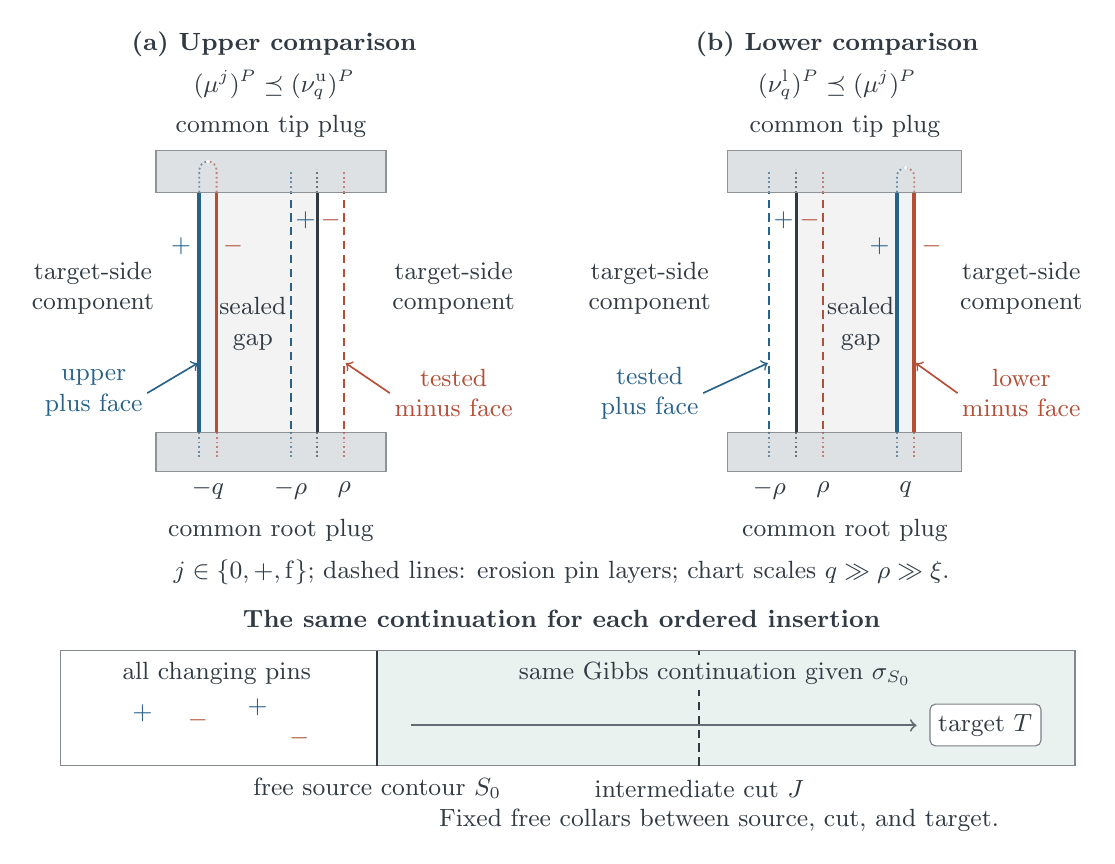
\begin{tikzpicture}[
  x=1cm,y=1cm,font=\small,text=slitink,
  wall/.style={draw=slitink,line width=1.15pt},
  plusface/.style={draw=slitplus,line width=1.35pt},
  minusface/.style={draw=slitminus,line width=1.35pt},
  pluslayer/.style={draw=slitplus,densely dashed,line width=.8pt},
  minuslayer/.style={draw=slitminus,densely dashed,line width=.8pt},
  plug/.style={fill=slitplug,draw=slitink!55,line width=.45pt},
  guide/.style={draw=slitink!60,line width=.45pt},
  ghost/.style={densely dotted,line width=.65pt,opacity=.65},
  every node/.style={inner sep=1.5pt,align=center}
]

\begin{scope}
  \node at (2.85,5.68) {\textbf{(a) Upper comparison}};
  \node at (2.85,5.16)
    {$(\mu^j)^P\preceq(\nu_q^{\mathrm u})^P$};

  \fill[slitink!6] (2.12,.60) rectangle (3.40,3.88);
  \node at (2.58,2.13) {sealed\\gap};
  \fill[slitplus!7] (1.90,.44) rectangle (2.12,4.04);
  \draw[plusface] (1.90,.44)--(1.90,4.04);
  \draw[minusface] (2.12,.44)--(2.12,4.04);
  \draw[wall] (3.40,.44)--(3.40,4.09);
  \draw[pluslayer] (3.06,.44)--(3.06,4.08);
  \draw[minuslayer] (3.74,.44)--(3.74,4.08);

  \node[text=slitplus] at (1.67,3.12) {$+$};
  \node[text=slitminus] at (2.33,3.12) {$-$};
  \node[text=slitplus] at (3.25,3.45) {$+$};
  \node[text=slitminus] at (3.57,3.45) {$-$};
  \node at (.55,2.58) {target-side\\component};
  \node at (5.13,2.58) {target-side\\component};

  \node[text=slitplus] (uplus) at (.56,1.25) {upper\\plus face};
  \draw[->,draw=slitplus,line width=.6pt]
    (uplus.east)--(1.88,1.63);
  \node[text=slitminus] (uminus) at (5.13,1.25) {tested\\minus face};
  \draw[->,draw=slitminus,line width=.6pt]
    (uminus.west)--(3.76,1.63);

  \draw[plug] (1.35,.25) rectangle (4.27,.75);
  \draw[plug] (1.35,3.80) rectangle (4.27,4.33);
  \node at (2.81,4.64) {common tip plug};
  \node at (2.81,-.49) {common root plug};
  \draw[ghost,draw=slitplus] (1.90,3.80)--(1.90,4.08)
    arc[start angle=180,end angle=90,radius=.11];
  \draw[ghost,draw=slitminus] (2.12,3.80)--(2.12,4.08)
    arc[start angle=0,end angle=90,radius=.11];
  \fill[white] (2.01,4.19) circle[radius=.025];
  \draw[ghost,draw=slitink] (3.40,3.80)--(3.40,4.09);
  \draw[ghost,draw=slitplus] (3.06,3.80)--(3.06,4.08);
  \draw[ghost,draw=slitminus] (3.74,3.80)--(3.74,4.08);
  \draw[ghost,draw=slitplus] (1.90,.75)--(1.90,.44);
  \draw[ghost,draw=slitminus] (2.12,.75)--(2.12,.44);
  \draw[ghost,draw=slitink] (3.40,.75)--(3.40,.44);
  \draw[ghost,draw=slitplus] (3.06,.75)--(3.06,.44);
  \draw[ghost,draw=slitminus] (3.74,.75)--(3.74,.44);

  \node at (2.01,.02) {$-q$};
  \node at (3.06,.02) {$-\rho$};
  \node at (3.74,.02) {$\rho$};
\end{scope}

\begin{scope}[shift={(7.10,0)}]
  \node at (2.90,5.68) {\textbf{(b) Lower comparison}};
  \node at (2.90,5.16)
    {$(\nu_q^{\mathrm l})^P\preceq(\mu^j)^P$};

  \fill[slitink!6] (2.38,.60) rectangle (3.66,3.88);
  \node at (3.20,2.13) {sealed\\gap};
  \fill[slitplus!7] (3.66,.44) rectangle (3.88,4.00);
  \draw[plusface] (3.66,.44)--(3.66,4.00);
  \draw[minusface] (3.88,.44)--(3.88,4.00);
  \draw[wall] (2.38,.44)--(2.38,4.09);
  \draw[pluslayer] (2.04,.44)--(2.04,4.08);
  \draw[minuslayer] (2.72,.44)--(2.72,4.08);

  \node[text=slitplus] at (3.44,3.12) {$+$};
  \node[text=slitminus] at (4.10,3.12) {$-$};
  \node[text=slitplus] at (2.22,3.45) {$+$};
  \node[text=slitminus] at (2.55,3.45) {$-$};
  \node at (.52,2.58) {target-side\\component};
  \node at (5.24,2.58) {target-side\\component};

  \node[text=slitplus] (lplus) at (.52,1.25) {tested\\plus face};
  \draw[->,draw=slitplus,line width=.6pt]
    (lplus.east)--(2.02,1.63);
  \node[text=slitminus] (lminus) at (5.24,1.25) {lower\\minus face};
  \draw[->,draw=slitminus,line width=.6pt]
    (lminus.west)--(3.90,1.63);

  \draw[plug] (1.51,.25) rectangle (4.48,.75);
  \draw[plug] (1.51,3.80) rectangle (4.48,4.33);
  \node at (3.00,4.64) {common tip plug};
  \node at (3.00,-.49) {common root plug};
  \draw[ghost,draw=slitplus] (3.66,3.80)--(3.66,4.00)
    arc[start angle=180,end angle=90,radius=.11];
  \draw[ghost,draw=slitminus] (3.88,3.80)--(3.88,4.00)
    arc[start angle=0,end angle=90,radius=.11];
  \fill[white] (3.77,4.11) circle[radius=.025];
  \draw[ghost,draw=slitink] (2.38,3.80)--(2.38,4.09);
  \draw[ghost,draw=slitplus] (2.04,3.80)--(2.04,4.08);
  \draw[ghost,draw=slitminus] (2.72,3.80)--(2.72,4.08);
  \draw[ghost,draw=slitplus] (3.66,.75)--(3.66,.44);
  \draw[ghost,draw=slitminus] (3.88,.75)--(3.88,.44);
  \draw[ghost,draw=slitink] (2.38,.75)--(2.38,.44);
  \draw[ghost,draw=slitplus] (2.04,.75)--(2.04,.44);
  \draw[ghost,draw=slitminus] (2.72,.75)--(2.72,.44);

  \node at (2.04,.02) {$-\rho$};
  \node at (2.72,.02) {$\rho$};
  \node at (3.77,.02) {$q$};
\end{scope}

\node at (6.50,-1.02)
  {$j\in\{0,+,\mathrm f\}$; dashed lines: erosion pin layers;
   chart scales $q\gg\rho\gg\xi$.};

\node at (6.50,-1.62) {\textbf{The same continuation for each ordered insertion}};
\fill[slitcollar] (4.16,-3.48) rectangle (13.02,-2.02);
\draw[guide] (.14,-3.48) rectangle (13.02,-2.02);
\node at (2.12,-2.31) {all changing pins};
\node[text=slitplus] at (1.18,-2.82) {$+$};
\node[text=slitminus] at (1.88,-2.91) {$-$};
\node[text=slitplus] at (2.64,-2.74) {$+$};
\node[text=slitminus] at (3.17,-3.13) {$-$};
\draw[draw=slitink,line width=.8pt] (4.16,-3.48)--(4.16,-2.02);
\draw[draw=slitink,densely dashed,line width=.8pt]
  (8.25,-3.48)--(8.25,-2.02);
\node[fill=slitcollar] at (8.45,-2.32)
  {same Gibbs continuation given $\sigma_{S_0}$};
\draw[->,draw=slitink!75,line width=.7pt] (4.59,-2.97)--(11.01,-2.97);
\draw[rounded corners=2pt,fill=white,draw=slitink!65]
  (11.18,-3.23) rectangle (12.59,-2.70);
\node at (11.88,-2.965) {target $T$};
\node at (4.16,-3.77) {free source contour $S_0$};
\node at (8.25,-3.77) {intermediate cut $J$};
\node at (8.50,-4.18)
  {Fixed free collars between source, cut, and target.};
\end{tikzpicture}%
}
\endgroup

\caption{Ordered comparison in a topological slit chart, and the common
continuation used for each insertion. The old slit has plus on its left
and minus on its right; the black tested wall has chart coordinate zero.
The displayed inequalities concern the laws restricted to the common
target component. In (a) the upper ribbon moves towards the plus
side; in (b) the lower ribbon moves towards the minus side. Common root
and tip plugs seal each interwall channel. All ends extend into the
plugs with slack; dotted cap traces show geometry overwritten by the
common plug assignment. The common free target component sees an upper
plus or tested minus face in (a), and a tested plus or lower minus face
in (b), or identical plug data. The exterior sectors may communicate
outside the chart. Dashed erosion layers may supply the tested frontier
after insertion; the opposite layer is screened. The lower strip shows
the shared source contour $S_0$, an intermediate cut $J$, and the target
$T$: all changed facing-boundary pins precede $S_0$, and for each fixed
distant wall the conditional continuation beyond it is the same. The
coordinates are chart coordinates, with $q\gg\rho\gg\xi$; no metric
regularity of the chart is assumed.}
\label{if:slit-figure}
\end{figure}

\emph{Incidence ordering for every nearby transcript.}
Let $\mu^0,\mu^+,\mu^{\mathrm f}$ be the three laws in the statement.
We compare their plugged versions to the same two plugged regular
laws. Figure~\ref{if:slit-figure} shows the local geometry. First
consider a slit strip outside the node plugs. Give the old slit plus
on its left and minus on its right, and put it at chart coordinate
$x=0$. The actual perturbed strand lies in $|x|<\xi$, where
$\xi\ll\rho$. The upper ribbon is near $x=-q$, the erosion plus
layer near $x=-\rho$, and the erosion minus layer near $x=\rho$.

Parametrized convergence also controls visits to the strip ends.
For each ideal edge, its part between the smaller node rectangles
lies in a strip separated from all nonincident edges. On the matched
perturbed edge, select its last exit from the first smaller rectangle
before its first entry into the second. This gives a simple crosscut.
The ideal edge is monotone near each node, so closeness of the
parametrizations places these exit and entry parameters near the
corresponding ideal parameters. The positive gap between the smaller
rectangle and the actual plug therefore keeps the entire discarded
prefix and suffix inside their respective plugs. For example, in a
local edge coordinate with smaller-rectangle exit at $s=2h$ and plug
exit at $s=3h$, a tolerance $e<h/3$ puts every point of the discarded
prefix at $s\le2h+2e<3h$.

Retain the entire selected crosscut, including any later visits to
an outer plug. Every portion of the original edge outside the actual
plugs is then retained. Turns and repeated plug visits do not change
the crosscut's separation of its two long sides: filling the plugs
can remove components but cannot join the two sides. Its orientation
identifies the accessible face signs, as in
Lemma~\ref{if:triangle-incidence}. This argument applies to every
slit and to each base arc between consecutive nodes. There are only
finitely many edges, so one tolerance works for all of them. Taking
the mesh below the remaining physical slack prevents a lattice edge
from passing between a wall end and its plug.

The upper ribbon and this old-wall crosscut, joined through the
wholly pinned root and tip plugs, close the channel between them.
That channel cannot meet the target component of the sites free in
both laws. Additional examined pieces cannot reopen it. The common
target component can consequently see only the plus face of the
upper ribbon or the minus face of the old wall. In the fully eroded
tested law, the latter frontier may instead be the erosion minus
layer. In the plus-only tested law, its extra plus pins lie in the
screened channel. The same upper comparison therefore works for
all three laws. Lemma~\ref{if:triangle-incidence} identifies each
accessible examined-neighbor sign with the appropriate wall face;
the recorded-data displacement was already absorbed into its
physical slack. At plug incidences the signs agree by construction.

For a base arc the verification is one-sided. If its sign is plus,
the upper outline is nearer the fresh side, so the upper model
supplies a plus pin at the common component's frontier. If its sign
is minus, the tested wall is nearer and supplies a minus pin. The
sign-changing joins are inside the common plugs. Thus every
incidence satisfies Lemma~\ref{if:incidence-order}, and
$ (\mu^j)^P\preceq(\nu_q^{\mathrm u})^P$ on the common target
component for $j\in\{0,+,\mathrm f\}$.

For the lower comparison move the ribbon to the minus side. The
accessible incidences are the lower minus face or the tested plus
face. Additional tested plus pins reinforce this order; the erosion
minus pins lie in the screened channel. The base-arc argument is
reversed in the same way, and the plugs again give identical signs.
Applying the incidence criterion proves the full sandwich
\begin{equation}\label{if:plugged-sandwich}
 (\nu_q^{\mathrm l})^P
       \preceq (\mu^j)^P
       \preceq (\nu_q^{\mathrm u})^P,
            \qquad j\in\{0,+,\mathrm f\}.
\end{equation}

\emph{Mean bounds and the completed law.}
Removing the plugs changes each mean by less than $a$. Thus
\eqref{if:plugged-sandwich} places every
$\mathbb E_{\mu^j}M_J^\delta$ between the two unmodified regular
means with error at most $2a$ at either end. Each of the two ordered
mean differences in \eqref{if:erosion-mean-reduction} is at most
the absolute regular mean gap plus $4a$. Choose $a$ first and then
$q$ so that Equation~\eqref{if:envelope-line-gap} and this error
make the sum of target total-variation changes less than
$\varepsilon$. All later choices of $\rho$, regularization,
neighborhood, and mesh preserved these bounds. No spin-scaling
limit in a realized transcript's irregular domain has been used.

Finally, the completed layer separates the target from every old
examined vertex. Conditional factorization of the Gibbs weights
therefore leaves exactly the law with the chosen new boundary and
the unchanged distant wall. It is independent of the transcript.
The argument conditions on the full transcript, including the
actual auxiliary radii when they are random. Omitted initial spins
and nonvisible traces lie on the blocked side of the new barrier.
A stopping radius producing no visible tip adds no boundary piece.
Thus the same completed law works even when the datum does not
record its numerical radii. Averaging over these radii or other
omitted information preserves the two total-variation bounds.
\end{proof}

\begin{lemma}[Moving a completed barrier outward]
\label{if:barrier-buffer}
In the inward setting, let a regular signed contour $\Gamma$
have already been fully pinned, and let $V^\delta$ be the entire
free component it encloses, with its pinned boundary layer excluded.
Assume that a positive exterior collar of $\Gamma$ contains no other
pins, as supplied by Lemma~\ref{if:erosion}.
For any compact target on its inner side and any $\varepsilon>0$,
one can choose a regular surrounding contour $\widehat\Gamma$
at a positive distance from $\Gamma$, with corresponding signs,
so that the following two steps on the marginal on $V^\delta$
each change the target law by less than $\varepsilon$:
\begin{enumerate}
\item remove the old plus pins on $\Gamma$;
\item remove the old minus pins on $\Gamma$.
\end{enumerate}
Here the farther pins on $\widehat\Gamma$ are present from the start.
They initially have no effect on $V^\delta$.  The first step is
downward and the second upward.  After both, the kept volume
$V^\delta$ is separated from every fixed pin by a positive
macroscopic distance, uniform for sufficiently fine meshes.
\end{lemma}

\begin{proof}
Choose $\widehat\Gamma$ as a sufficiently thin outward offset of
$\Gamma$, matching the finite sign arcs.  Put the new pins there
before changing the old ones.  The full old layer disconnects the
kept volume, so these farther pins are initially harmless.  We
retain the same $V^\delta$ throughout the argument; in particular
we do not first discard a free strip inside the old layer.

Use the construction of Lemma~\ref{if:erosion} without slits.
Put small identical plugs around the finitely many sign switches,
make upper and lower regular outlines by moving plus and minus
arcs in their respective ordered directions, and compare by
Lemma~\ref{if:incidence-order}.  The test contour lies strictly
inside $\Gamma$, with a common free collar.  As the offset tends
to zero, both unmodified envelope means have the same limit by
Lemma~\ref{if:marked-convergence}; the plug errors tend to zero
by Corollary~\ref{fd:patch-ratio}.  This controls the means for the
original law, the law with only the old minus pins remaining,
and the law with all old pins removed.  The two actual removals
are ordered, so Corollary~\ref{tr:ordered-tv} proves the claimed
target estimates.

Fix the sufficiently small offset after obtaining these estimates.
Its physical distance from $\Gamma$ is positive, and mesh rounding
preserves a fixed fraction of it.  The kept volume is inside
$\Gamma$; the effective boundary pins are on the farther contour,
and the original pins are farther away, beyond the available collar.
This proves the final buffer assertion.
\end{proof}
